\begin{itemize}
    \item Differential equation~\eqref{eq:odd-exponential-identity} can also be expressed in terms of backward
    and central differential operators, including derivatives on time-scales so that results of~\cite{kolosov2016study}
    could be generalized further.
    \item Theorem~\eqref{eq:odd-power-theorem} gives an opportunity to express odd-power identity
    in terms of multiplication of certain matrices.
    \item There are Taylor series and Maclaurin series versions in terms of $\polynomialP{m}{b}{x}$.
    \item Definition~\eqref{eq:definition_polynomial_p} is closely related to discrete convolution because
    \begin{equation*}
        \polynomialP{m}{b}{x} = \sum_{r=0}^{m} \coeffA{m}{r} \sum_{k=0}^{b-1} k^r(x-k)^r
    \end{equation*}
    where $\sum_{k=0}^{b-1} k^r(x-k)^r$ is the discrete convolution of $x^r$.
    It is worth to get a closer look at it so that new relations in terms of discrete convolution may be found.
    \item All kinds of derivatives e.g forward, backward and central, including the derivatives on time-scales can be expressed
    as double limit of $\polynomialP{m}{b}{x}$ extending the results of~\cite{kolosov_2024_10575485}.
    \item Introducing the definition of coefficient $\llceilCoefficient{m,n}{k}$
    \begin{equation*}
        \llceilCoefficient{m,n}{k} = \sum_{r=0}^{m} \coeffA{m}{r} k^r (n-k)^r
    \end{equation*}
    the novel identities can be reached, for example
    \begin{align*}
        \llceilCoefficient{m, 2t+1}{1} &= \llceilCoefficient{m, t+2}{2} \\
        \llceilCoefficient{m, n}{k} &= \llceilCoefficient{m, n}{n-k} \\
        \llceilCoefficient{m, 2t-3r}{r} &= \llceilCoefficient{m, t}{2r} = \llceilCoefficient{m, 2t-3r}{2t-4r}
    \end{align*}
    so that combinatorial sense of above is also a topic to research.
    \item Following the results of~\url{https://arxiv.org/pdf/1603.02468v15.pdf},
    the equation~\eqref{eq:definition_polynomial_p} approximates the odd-power polynomial $x^{2m+1}$ around given points
    $x_i$ as it may be observed from the following plots
    \begin{figure}[H]
        \centering
        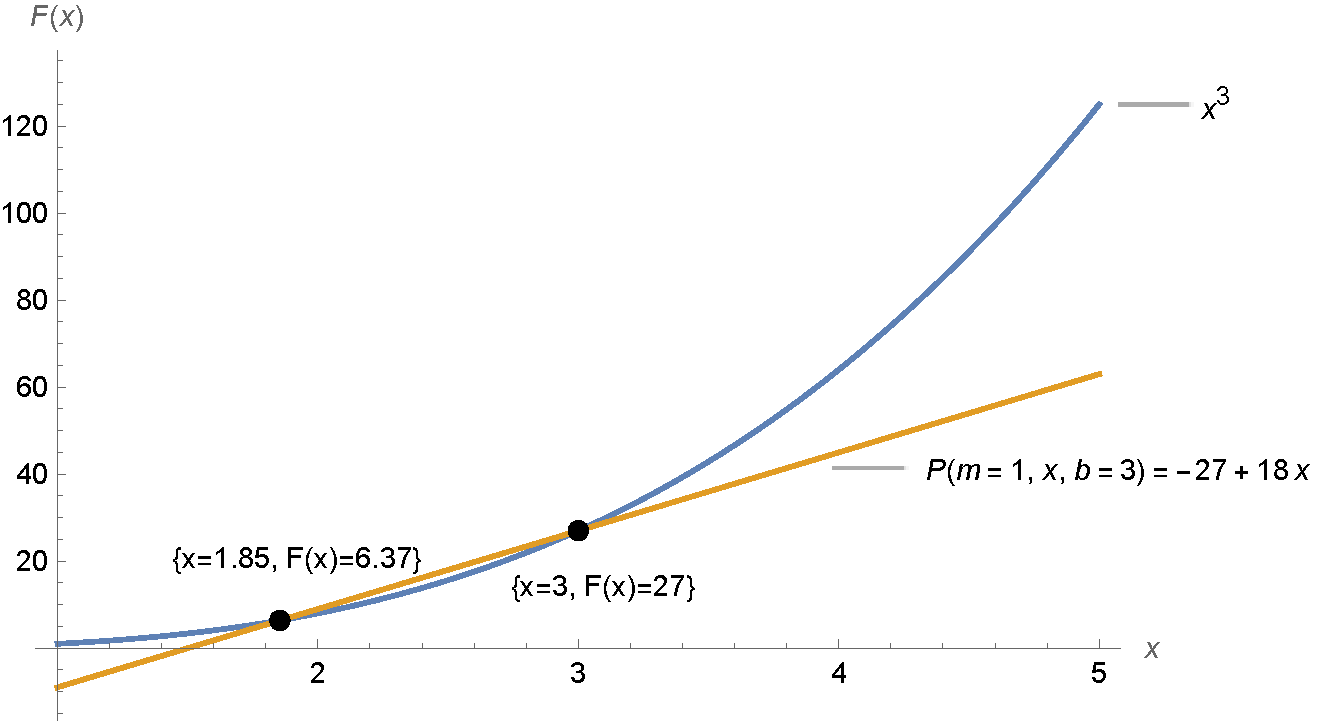
\includegraphics[width=1\textwidth]{images/n^3_approximation_m1_b3}
        ~\caption{Approximation of $x^3$.}\label{fig:approximation-n3}
    \end{figure}
    \begin{figure}[H]
        \centering
        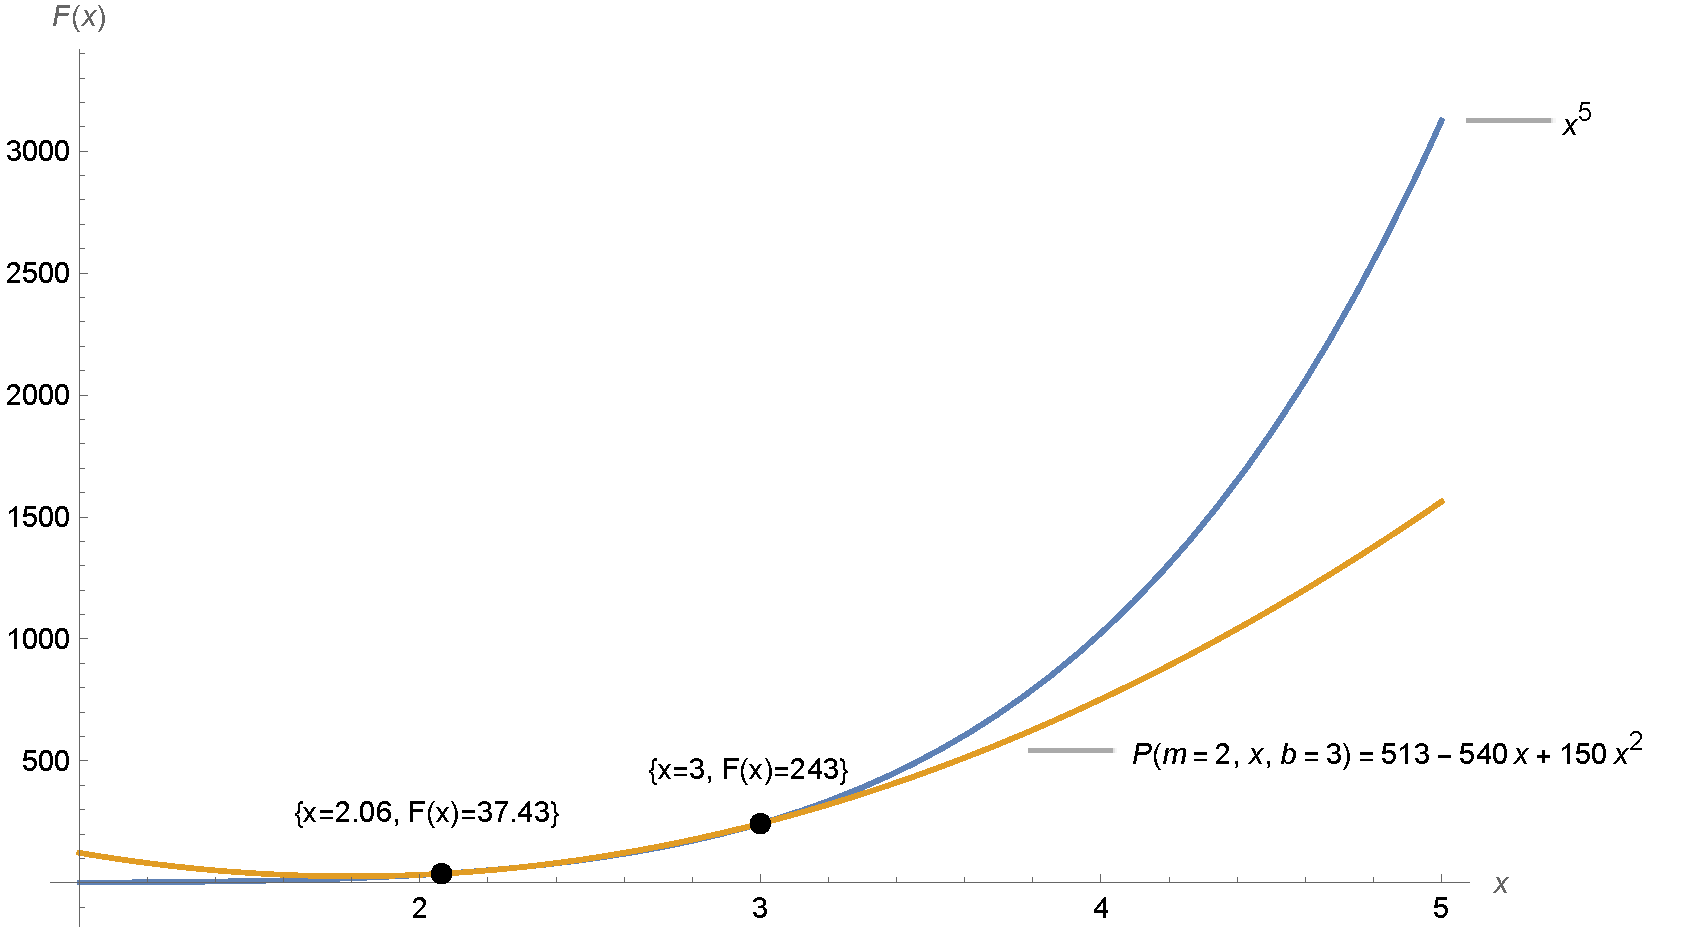
\includegraphics[width=1\textwidth]{images/n^5_approximation_m2_b3}
        ~\caption{Approximation of $x^5$.}\label{fig:approximation-n5}
    \end{figure}
    \item English grammar reviews and improvements are welcome.
    \item Improvements and suggestions to current manuscript under open-source initiatives at
    \url{https://github.com/kolosovpetro/HistoryAndOverviewOfPolynomialP}
\end{itemize}
